%%%%%%%%%%%%%%%%%%%%%%%%%%%%%%%%%%%%%%%%%
% Beamer Presentation
% LaTeX Template
% Version 1.0 (10/11/12)
%
% This template has been downloaded from:
% http://www.LaTeXTemplates.com
%
% License:
% CC BY-NC-SA 3.0 (http://creativecommons.org/licenses/by-nc-sa/3.0/)
%
%%%%%%%%%%%%%%%%%%%%%%%%%%%%%%%%%%%%%%%%%

%----------------------------------------------------------------------------------------
%	PACKAGES AND THEMES
%----------------------------------------------------------------------------------------

%\documentclass[UTF8,aspectratio=169,14pt]{ctexbeamer}
\documentclass[UTF8,aspectratio=169]{ctexbeamer}
\usepackage{hyperref}
\hypersetup{
	colorlinks=true,
	linkcolor=red,
	anchorcolor=blue,
	citecolor=green
}

\mode<presentation> {
	
	% The Beamer class comes with a number of default slide themes
	% which change the colors and layouts of slides. Below this is a list
	% of all the themes, uncomment each in turn to see what they look like.
	
	%\usetheme{default}
	%\usetheme{AnnArbor}
	%\usetheme{Antibes}
	%\usetheme{Bergen}
	%\usetheme{Berkeley}
	%\usetheme{Berlin}
	%\usetheme{Boadilla}
	%\usetheme{CambridgeUS}
	%\usetheme{Copenhagen}
	%\usetheme{Darmstadt}
	%\usetheme{Dresden}
	%\usetheme{Frankfurt}
	%\usetheme{Goettingen}
	%\usetheme{Hannover}
	%\usetheme{Ilmenau}
	%\usetheme{JuanLesPins}
	%\usetheme{Luebeck}
	\usetheme{Madrid}
	%\usetheme{Malmoe}
	%\usetheme{Marburg}
	%\usetheme{Montpellier}
	%\usetheme{PaloAlto}
	%\usetheme{Pittsburgh}
	%\usetheme{Rochester}
	%\usetheme{Singapore}
	%\usetheme{Szeged}
	%\usetheme{Warsaw}
	
	% As well as themes, the Beamer class has a number of color themes
	% for any slide theme. Uncomment each of these in turn to see how it
	% changes the colors of your current slide theme.
	
	%\usecolortheme{albatross}
	%\usecolortheme{beaver}
	%\usecolortheme{beetle}
	%\usecolortheme{crane}
	%\usecolortheme{dolphin}
	%\usecolortheme{dove}
	%\usecolortheme{fly}
	%\usecolortheme{lily}
	%\usecolortheme{orchid}
	%\usecolortheme{rose}
	%\usecolortheme{seagull}
	%\usecolortheme{seahorse}
	%\usecolortheme{whale}
	%\usecolortheme{wolverine}
	
	%\setbeamertemplate{footline} % To remove the footer line in all slides uncomment this line
	%\setbeamertemplate{footline}[page number] % To replace the footer line in all slides with a simple slide count uncomment this line
	
	%\setbeamertemplate{navigation symbols}{} % To remove the navigation symbols from the bottom of all slides uncomment this line
}

\usepackage{graphicx} % Allows including images
\graphicspath{{./figs/}}
\usepackage{booktabs} % Allows the use of \toprule, \midrule and \bottomrule in tables
\usepackage{longtable}
\usepackage{listings}
\usepackage{xcolor}
\lstset{numbers=left, %设置行号位置
	numberstyle=\tiny, %设置行号大小
	keywordstyle=\color{blue}, %设置关键字颜色
	commentstyle=\color[cmyk]{1,0,1,0}, %设置注释颜色
	frame=single, %设置边框格式
	escapeinside=``, %逃逸字符(1左面的键),用于显示中文
	%breaklines, %自动折行
	extendedchars=false, %解决代码跨页时,章节标题,页眉等汉字不显示的问题
	xleftmargin=2em,xrightmargin=2em, aboveskip=1em, %设置边距
	tabsize=4, %设置tab空格数
	showspaces=false %不显示空格
}
% Fonts
% \usepackage{libertine}
% \setmonofont{Courier}
\setCJKsansfont[ItalicFont=Noto Serif CJK SC Black, BoldFont=Noto Sans CJK SC Black]{Noto Sans CJK SC}
\setmainfont[Ligatures={Common,TeX}]{Linux  Libertine O}
\setmonofont[SmallCapsFont={Latin Modern Mono Caps}]{Latin Modern Mono Light}
\setsansfont{Linux Biolinum O}

\logo{
\includegraphics[width=0.55cm,height=0.55cm]{../../thcs-logo.png}}

%----------------------------------------------------------------------------------------
%	TITLE PAGE
%----------------------------------------------------------------------------------------

\title[第3讲]{第3讲 :Virtual Machine Monitor} % The short title appears at the bottom of every slide, the full title is only on the title page
\subtitle{第三节:Hardware-assisted Virtualization}
\author{陈渝} % Your name
\institute[清华大学] % Your institution as it will appear on the bottom of every slide, may be shorthand to save space
{
	清华大学计算机系 \\ % Your institution for the title page
	\medskip
	\textit{yuchen@tsinghua.edu.cn} % Your email address
}
\date{\today} % Date, can be changed to a custom date


\begin{document}

\begin{frame}
\titlepage % Print the title page as the first slide
\end{frame}

%\begin{frame}
%\frametitle{提纲} % Table of contents slide, comment this block out to remove it
%\tableofcontents % Throughout your presentation, if you choose to use \section{} and \subsection{} commands, these will automatically be printed on this slide as an overview of your presentation
%\end{frame}
%
%%----------------------------------------------------------------------------------------
%%	PRESENTATION SLIDES
%%----------------------------------------------------------------------------------------
%
%%------------------------------------------------
%\section{第一节:课程概述} % Sections can be created in order to organize your presentation into discrete blocks, all sections and subsections are automatically printed in the table of contents as an overview of the talk
%%------------------------------------------------

%-------------------------------------------------
\begin{frame}[plain]
	\frametitle{Problems }
	
	
	
	\begin{columns}
		
		\begin{column}{.3\textwidth}
			
			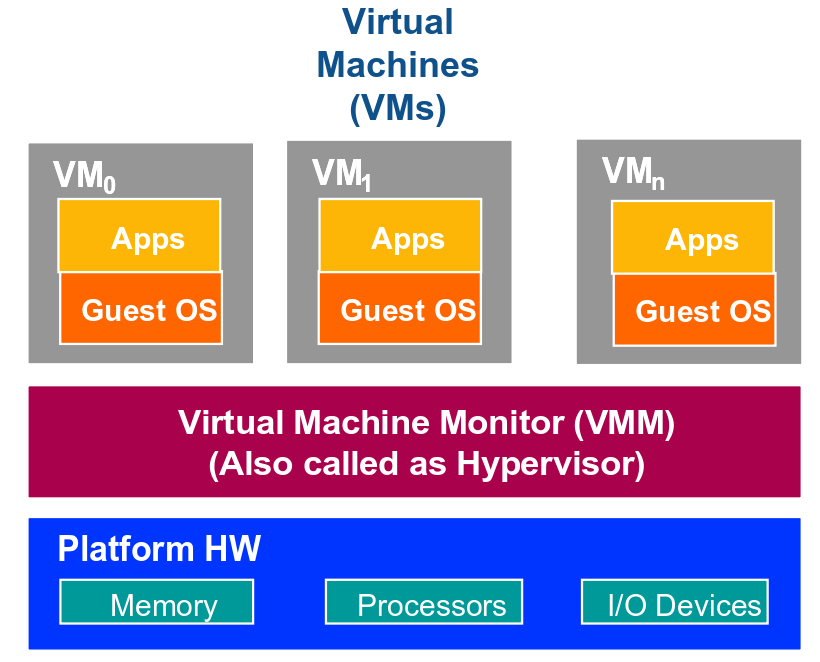
\includegraphics[width=1.\textwidth]{vmm-overview}
			
		\end{column}
		
		\begin{column}{.7\textwidth}
			
			\textbf{Virtualization holes}

		 Conventional Intel® 64, or IA-32, is not virtualizable architecture
			\begin{itemize}
				\item Sensitive register instructions: read or change sensitive registers and/or memory locations such as a clock register or interrupt registers

					\begin{itemize}
					\item  SGDT, SIDT, SLDT
					\item  SMSW 
					\item PUSHF, POPF 
					
					\end{itemize} 
				\item Protection system instructions: reference the storage protection system, memory or address relocation system
			
					\begin{itemize}
					\item  LAR, LSL, VERR, VERW 
					\item  POP, PUSH
					\item  CALL, JMP, INT n, RET 
					\item STR, MOVE
					\end{itemize} 
		
			\end{itemize} 
				\tiny Source from proceeding of 2000 USENIX ATC
		\end{column}
		
		
	\end{columns}
	
	
\end{frame}


%-------------------------------------------------
\begin{frame}[plain]
	\frametitle{Problems}
	
	
	
	\begin{columns}
		
		\begin{column}{.3\textwidth}
			
			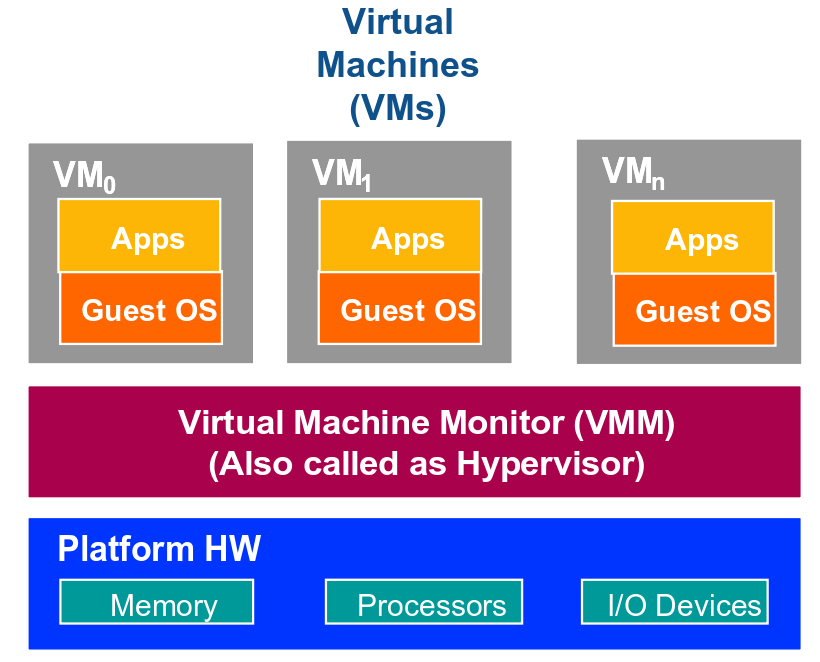
\includegraphics[width=1.\textwidth]{vmm-overview}
			
		\end{column}
		
		\begin{column}{.7\textwidth}
			
			\textbf{Controlling the CPU Resource}
			
			With an Intel® 64 CPU, a VMM must be able to retain control over
			\begin{itemize}
				\item Access to privileged state (CRn, DRn, MSRs)
				\item Exceptions (\#PF, \#MC, etc.)
				\item Interrupts and interrupt masking
				\item Address translation (via page tables)
				\item CPU access to I/O (via I/O ports or MMIO)
			\end{itemize} 

		\end{column}
		
		
	\end{columns}
	
	
\end{frame}

%-------------------------------------------------
\begin{frame}[plain]
	\frametitle{Problems }
	
	
	
	\begin{columns}
		
		\begin{column}{.3\textwidth}
			
			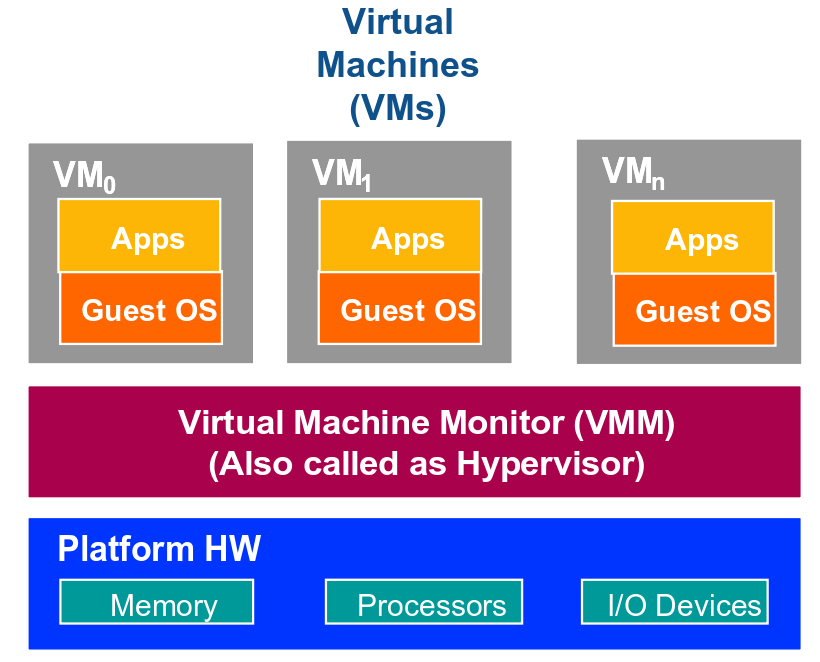
\includegraphics[width=1.\textwidth]{vmm-overview}
			
		\end{column}
		
		\begin{column}{.7\textwidth}
			
			\textbf{CPU Control via “Ring Deprivileging”}
			
			With an Intel® 64 CPU, a VMM must be able to retain control over
			\begin{itemize}
				\item Guest OS kernel runs in a less privileged ring than usual
				
				\item VMM runs in the most privileged ring 0
				\item prevent guest OS from accessing privileged instructions / state
				\item prevent guest OS from modifying VMM code and data

			\end{itemize} 
			
		\end{column}
		
		
	\end{columns}
	
	
\end{frame}


%-------------------------------------------------
\begin{frame}[plain]
	\frametitle{Problems }
	
	
	
	\begin{columns}
		
		\begin{column}{.3\textwidth}
			
			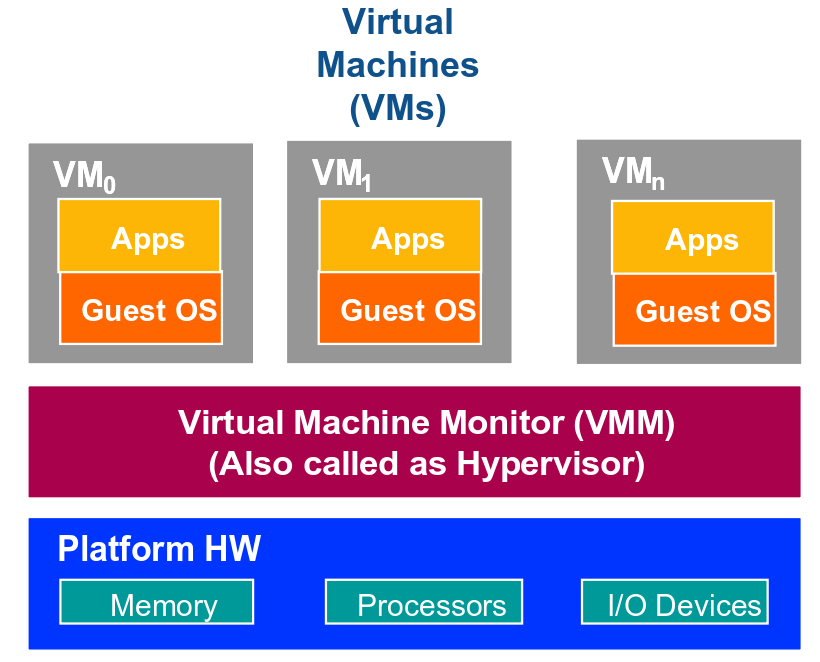
\includegraphics[width=1.\textwidth]{vmm-overview}
			
		\end{column}
		
		\begin{column}{.7\textwidth}
			
			\textbf{Problems with Ring Deprivileging}
			
			Ring deprivileging encounters various issues in current Intel® 64 architecture:
			\begin{itemize}
				\item Ring compression/aliasing
				\item Non-faulting reads of privileged state
				\item Excessive faulting
				\item Interrupt-virtualization issues
				
			\end{itemize} 
			
		\end{column}
		
		
	\end{columns}
	
	
\end{frame}


%-------------------------------------------------
\begin{frame}[plain]
	\frametitle{Solutions }
	
	
	
	\begin{columns}
		
		\begin{column}{.3\textwidth}
			
			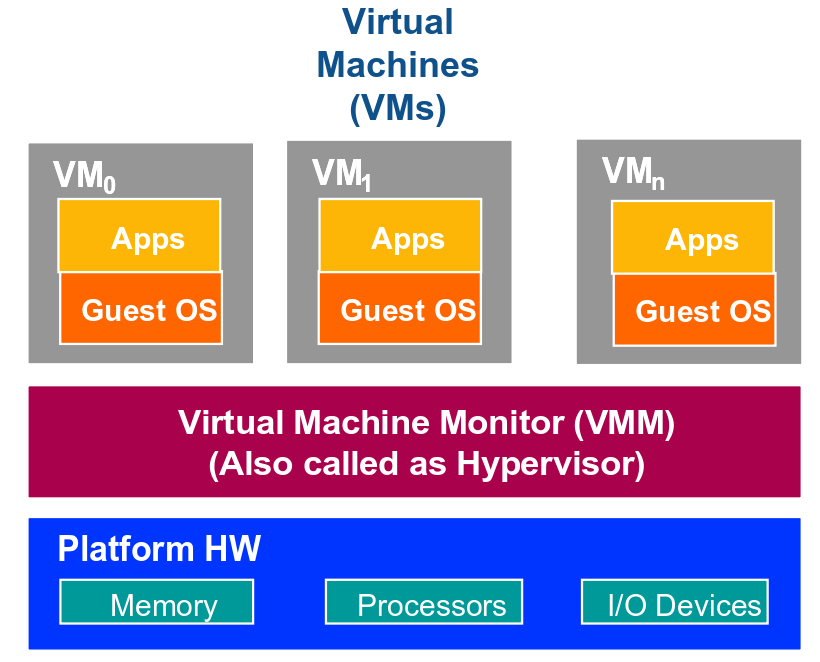
\includegraphics[width=1.\textwidth]{vmm-overview}
			
		\end{column}
		
		\begin{column}{.7\textwidth}
			
			\textbf{Addressing  “Virtualization Holes”}
			
			\begin{itemize}
				\item Paravirtualization
				\item Binary translation (or patching)
				\item Hardware-assisted virtualization
				\begin{itemize}
								
				\item Closing virtualization holes in hardware
				\item Simplify VMM software
				\item Optimizing for performance
				\end{itemize} 
			\end{itemize} 
			
		\end{column}
		
		
	\end{columns}
	
	
\end{frame}


%-------------------------------------------------
\begin{frame}[plain]
	\frametitle{Solution -- hardware-assisted VT }
	
	
	
	\begin{columns}
		
		\begin{column}{.3\textwidth}
			
			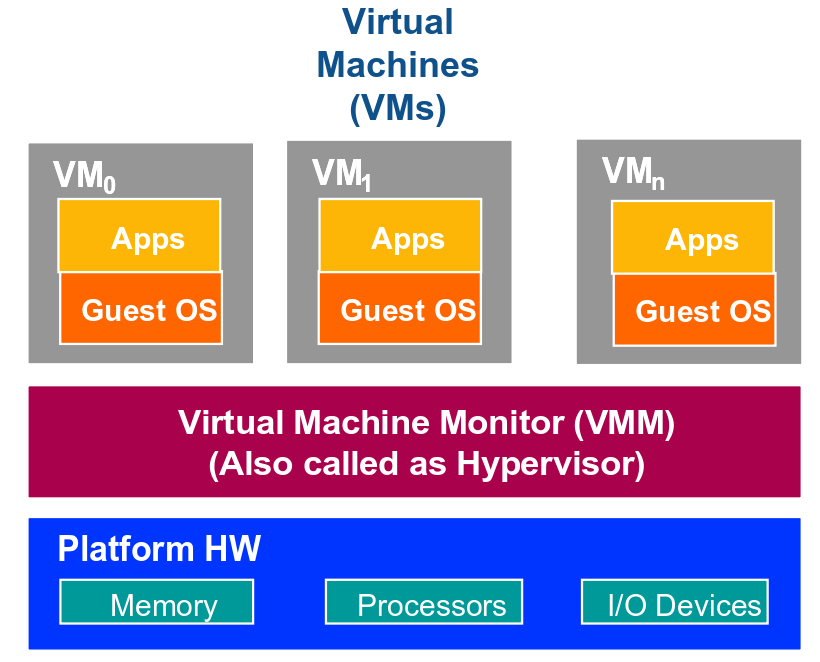
\includegraphics[width=1.\textwidth]{vmm-overview}
			
		\end{column}
		
		\begin{column}{.7\textwidth}
			
			\textbf{Intel® Virtualization Technology}
			
			A hardware-assisted virtualization technology, named as Intel® Virtualization Technology, or Intel® VT 
			\begin{itemize}
				\item For Intel® 64, VT-x: CPU MEM
				\item For directed I/O, VT-d: DMA/Interrupt remapping
				\item For connectivity, VT-c: offload wor from CPU to IO device

			\end{itemize} 
			
		\end{column}
		
		
	\end{columns}
	
	
\end{frame}

%-------------------------------------------------
\begin{frame}[plain]
	\frametitle{VT-x -- cpu}
	
	
	
	\begin{columns}
		
		\begin{column}{.5\textwidth}
			
			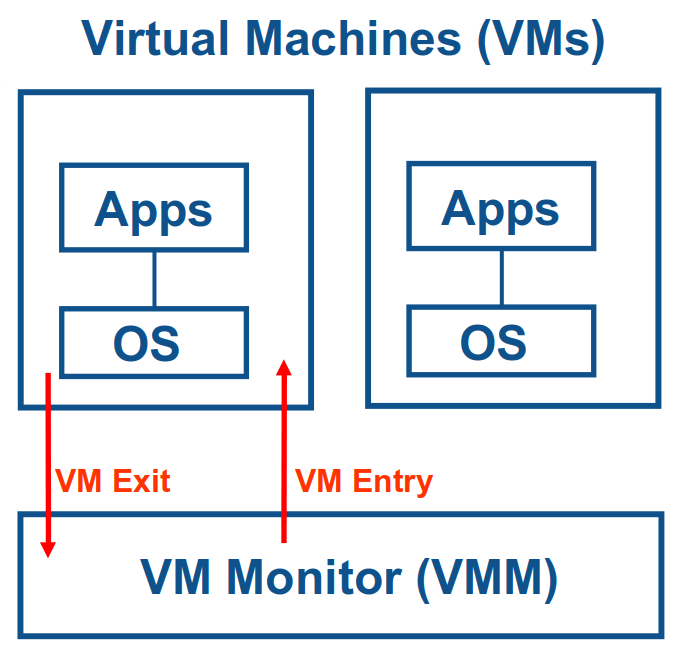
\includegraphics[width=.8\textwidth]{vmx-overview}
			
		\end{column}
		
		\begin{column}{.5\textwidth}
			
			\textbf{VM entry}
			
			\begin{itemize}
				\item Transition from VMM to guest
				\item Enters VMX non-root operation
				\item VMLAUNCH used for initial entry
				\item VMRESUME used subsequently
				
			\end{itemize} 
			
			\textbf{VM exit}
			
			\begin{itemize}
				\item Guest-to-VMM transition
				\item Enters VMX root operation
				\item Caused by external events,
				exceptions, some instructions

				
			\end{itemize} 
			
		\end{column}
		
		
	\end{columns}
	
	
\end{frame}

%-------------------------------------------------
\begin{frame}[plain]
	\frametitle{VT-x -- cpu}
	
	
	
	\begin{columns}
		
		\begin{column}{.5\textwidth}
			
			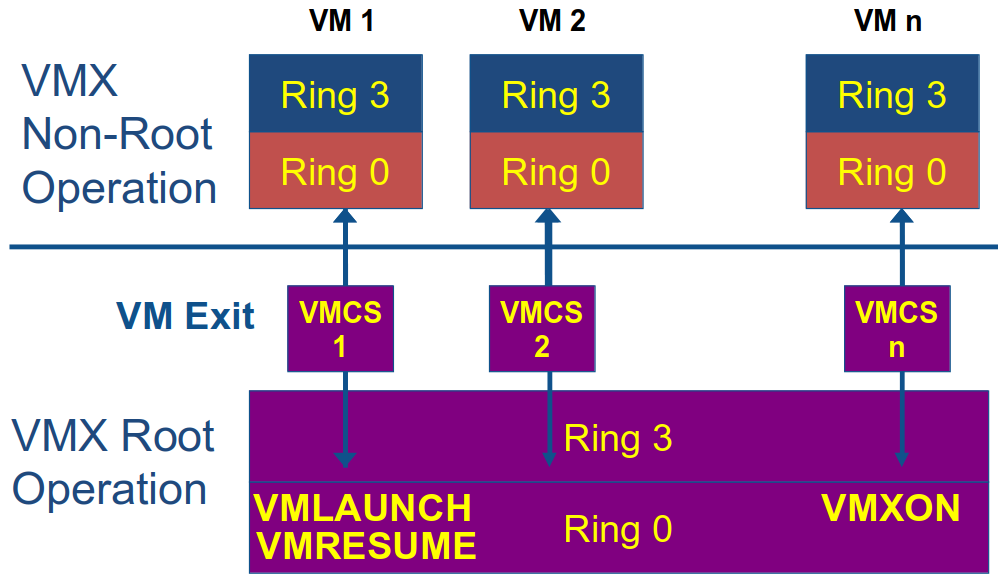
\includegraphics[width=1.\textwidth]{vt-x}
			
		\end{column}
		
		\begin{column}{.5\textwidth}
			
			\textbf{Virtual Machine Control Structure (VMCS)}
			
%			\hline
			Controls VMX non-root operation/transitions
			\begin{itemize}
				\item Each virtual CPU should have its own VMCS
				\item Only one VMCS active at a time on a physical CPU
				
			\end{itemize} 
			
			Each VMCS stored in a memory region
			
			\begin{itemize}
				\item Physical address set by new VMPTRLD instruction
				\item Need not reside in linear-address space 
				\item VMPTRLD also used to switch VMCS
				
				
			\end{itemize}
			
		\end{column}
		
		
	\end{columns}
	
	
\end{frame}

%-------------------------------------------------
\begin{frame}[plain]
	\frametitle{VT-x -- mem}
	
	
	
	\begin{columns}
		
		\begin{column}{.5\textwidth}
			
			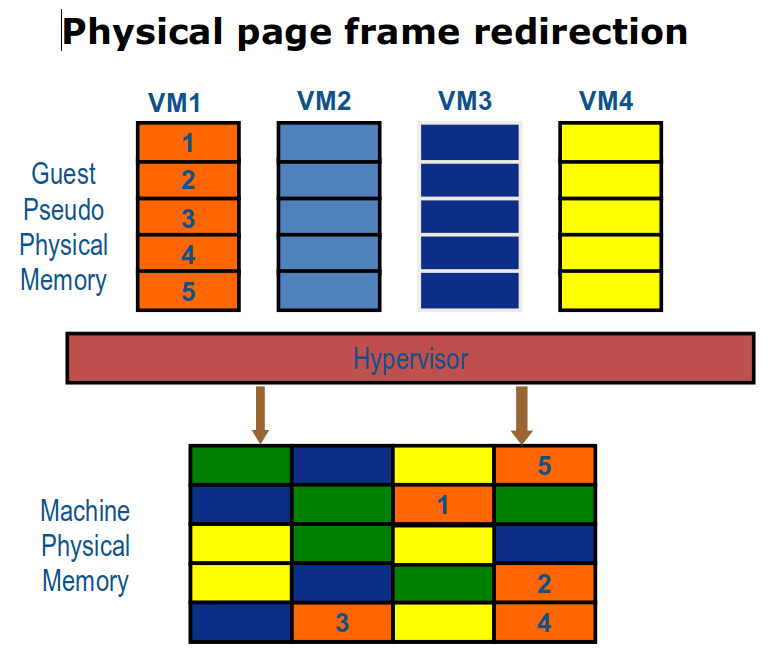
\includegraphics[width=1.\textwidth]{vt-x-mem}
			
		\end{column}
		
		\begin{column}{.5\textwidth}
			
			\textbf{Memory virtualization challenges}
			
%			\hline
			
			\begin{itemize}
				\item OS expect to see physical memory starting from 0
				\item OS expect to see contiguous memory in address space
				\item BIOS/Legacy OS are designed to boot from address low 1M
				\item DMA, TLB, etc.
			\end{itemize} 
			
			
			
		\end{column}
		
		
	\end{columns}
	
	
\end{frame}

%-------------------------------------------------
\begin{frame}[plain]
	\frametitle{VT-x -- mem}
	
			
			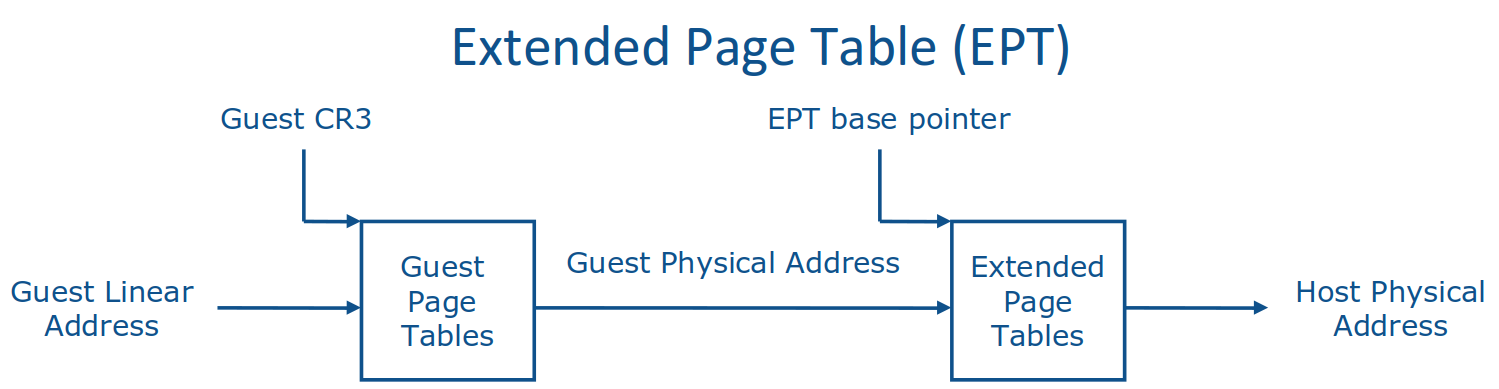
\includegraphics[width=1.\textwidth]{vt-x-ept}
		

			\textbf{Memory virtualization challenges}
			
			

			\begin{itemize}
				\item Guest can have full control over its page tables and events: 
				\begin{itemize}
				\item 	CR3, INVLPG, page fault
				\end{itemize}
				\item VMM controls Extended Page Tables:
				\begin{itemize}
				\item BIOS/Legacy OS are designed to boot from address low 1M
				\item DMA, TLB, etc.
				\end{itemize}
			\end{itemize} 
		
	
\end{frame}

%-------------------------------------------------
\begin{frame}[plain]
	\frametitle{VT-d}
	

	\begin{columns}
	
	\begin{column}{.4\textwidth}
		
		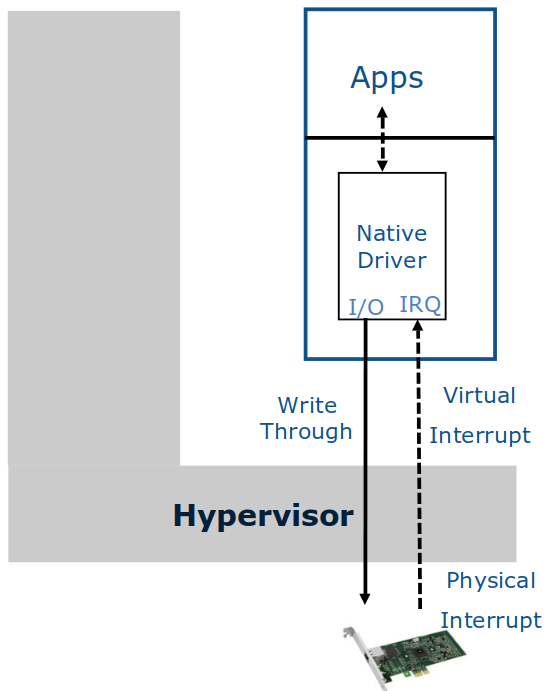
\includegraphics[width=1.\textwidth]{vt-d-direct}
		
	\end{column}
	
	\begin{column}{.5\textwidth}
		
	\textbf{Direct assignment}
	
	
	
	\begin{itemize}
		\item Guest runs native driver  
		\item I/O is written through
		\item Physical interrupt is captured by hypervisor (pIRQ)
		\item Virtual interrupt is signaled for guest (vIRQ)
		\item Remapping from pIRQ <-> vIRQ in hypervisor
	\end{itemize} 
	
	\textbf{Maximizing performance, but sacrificing sharing}
	
    \end{column}


\end{columns}
	
\end{frame}


%-------------------------------------------------
\begin{frame}[plain]
	\frametitle{VT-d}
	
	\centering
	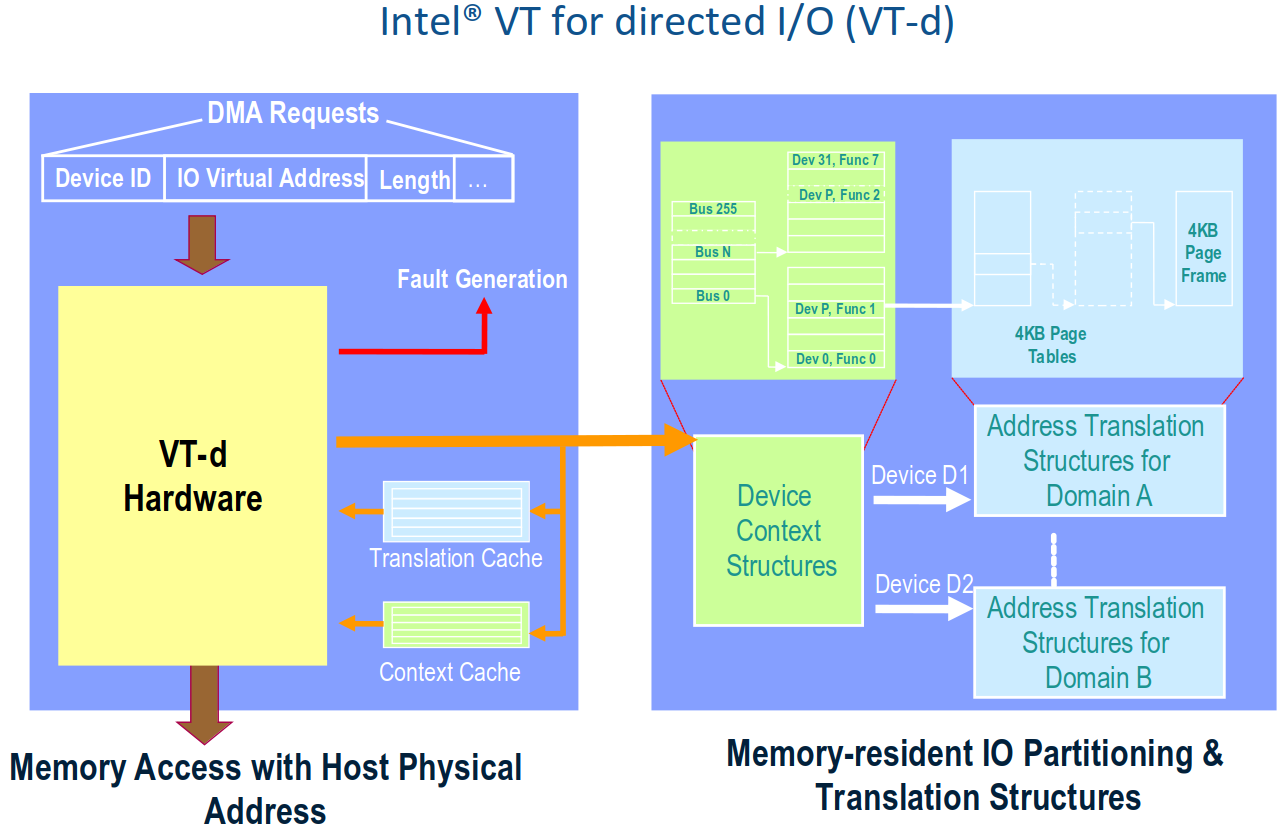
\includegraphics[width=.8\textwidth]{vt-d-overview}
	
	
	\textbf{Memory virtualization challenges}
	
	
	
\end{frame}

%-------------------------------------------------
\begin{frame}[plain]
	\frametitle{VT-c}
	
	
	\begin{columns}
		
		\begin{column}{.5\textwidth}
			
			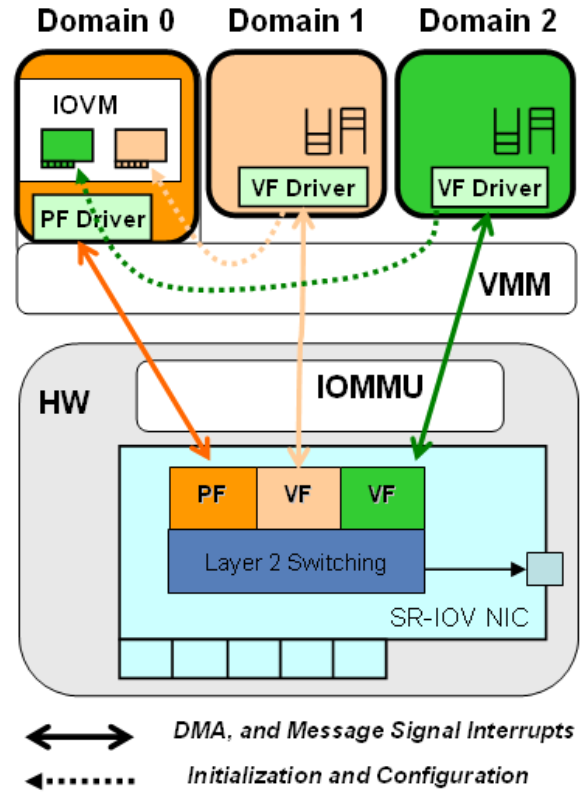
\includegraphics[width=.75\textwidth]{sriov}
			
		\end{column}
		
		\begin{column}{.5\textwidth}
			
			\textbf{Single Root I/O Virtualization (SR-IOV)}
			
			
			
			\begin{itemize}
				\item Close to native performance  
				\item Limited CPU overhead
				\item Flexible sharing
				\item Security control through PF
			\end{itemize} 
			
			\textbf{Maximizing performance}
			
		\end{column}
		
		
	\end{columns}
	
\end{frame}
%-------------------------------------------------
%-------------------------------------------------
\begin{frame}[plain]
	\frametitle{Summary}
	\centering
	
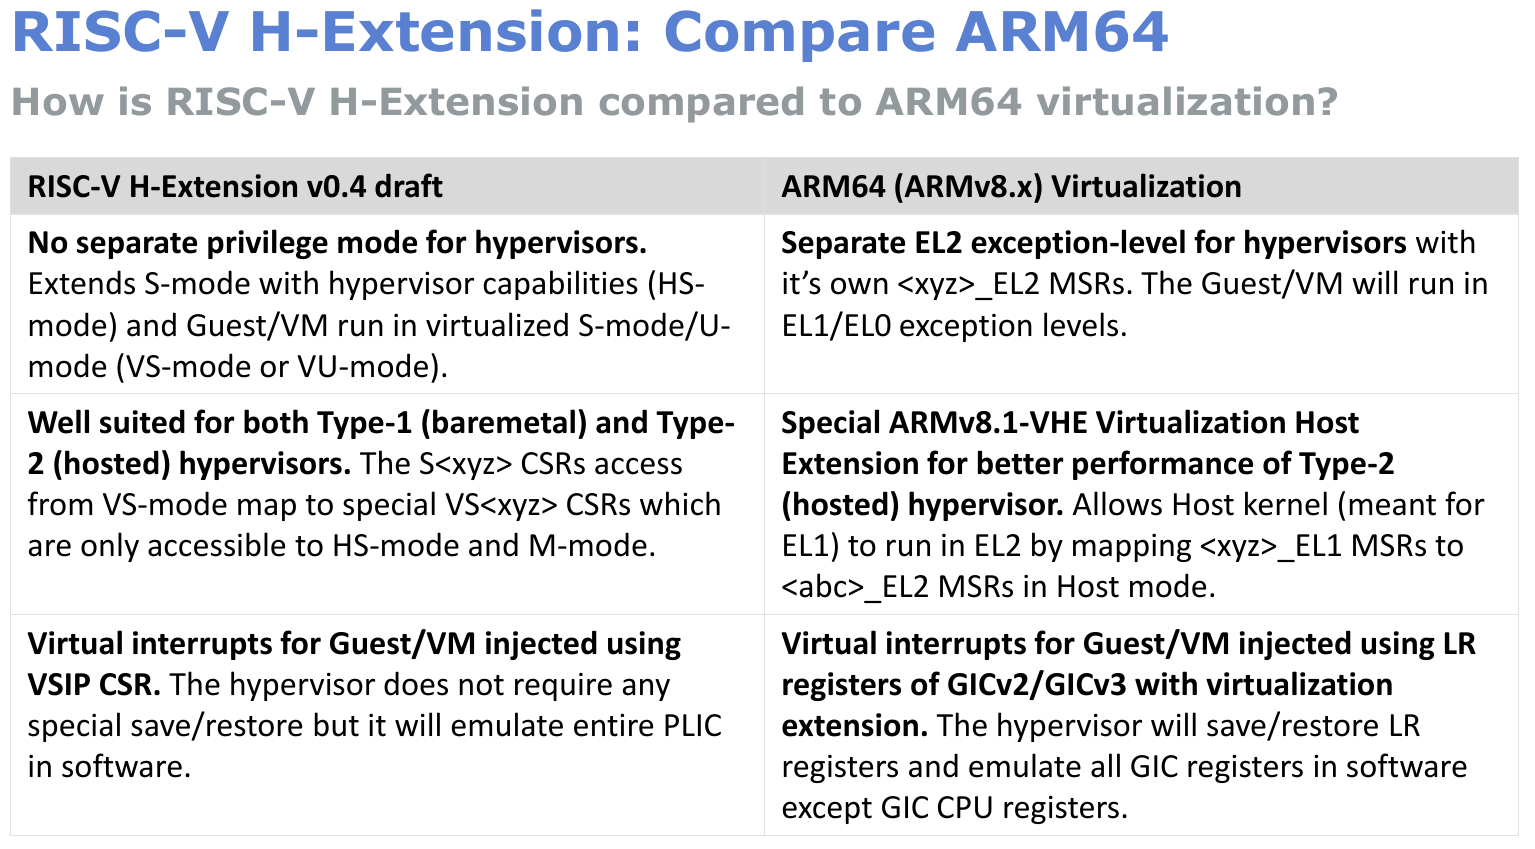
\includegraphics[width=.9\textwidth]{rv-arm-1}
	
\end{frame}

%-------------------------------------------------
\begin{frame}[plain]
	\frametitle{Summary}
	\centering
	
	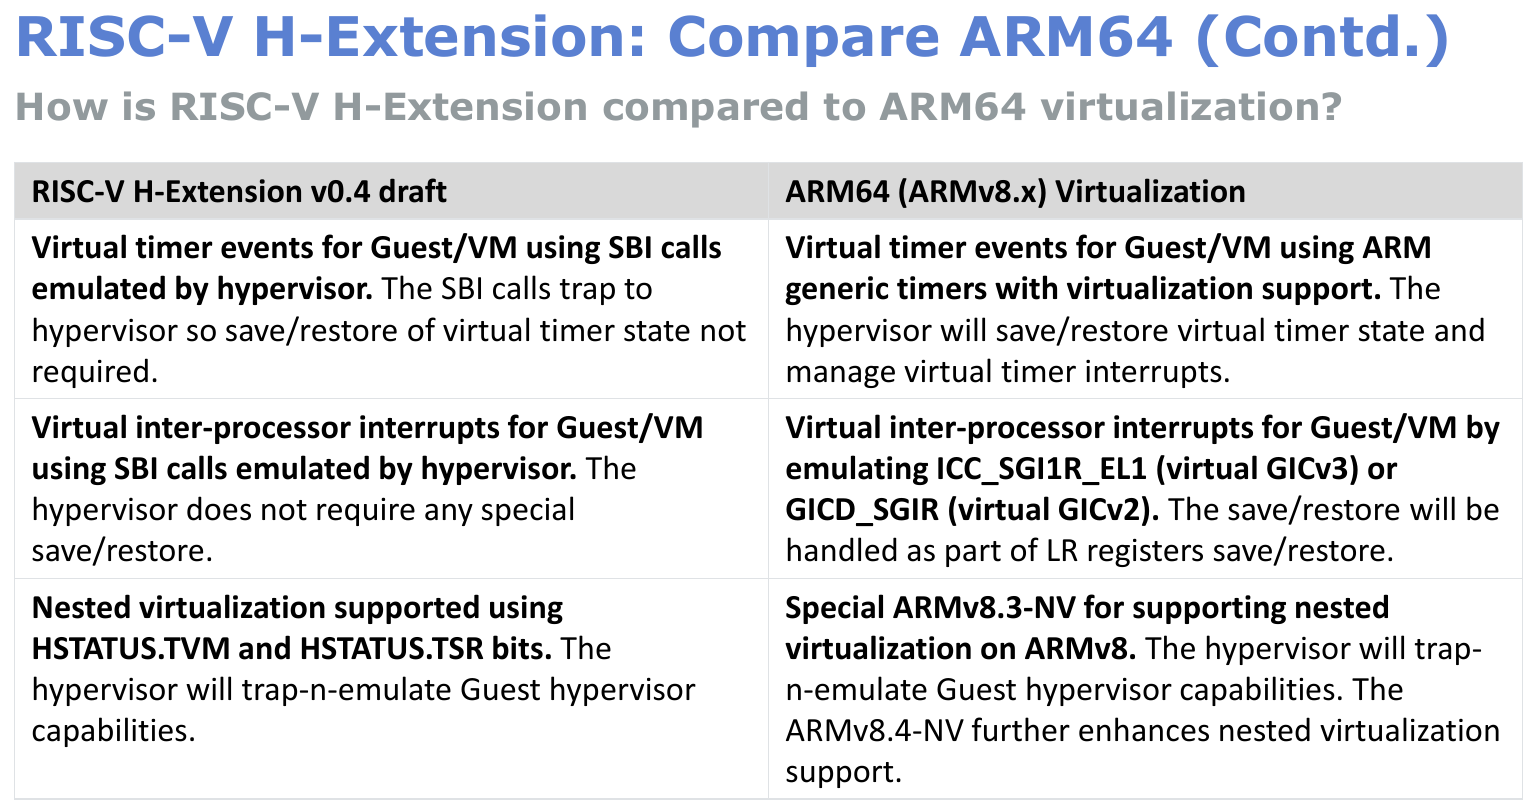
\includegraphics[width=.9\textwidth]{rv-arm-2}
	
\end{frame}


%-------------------------------------------------
\begin{frame}[plain]
	\frametitle{Summary}
	\centering
	
	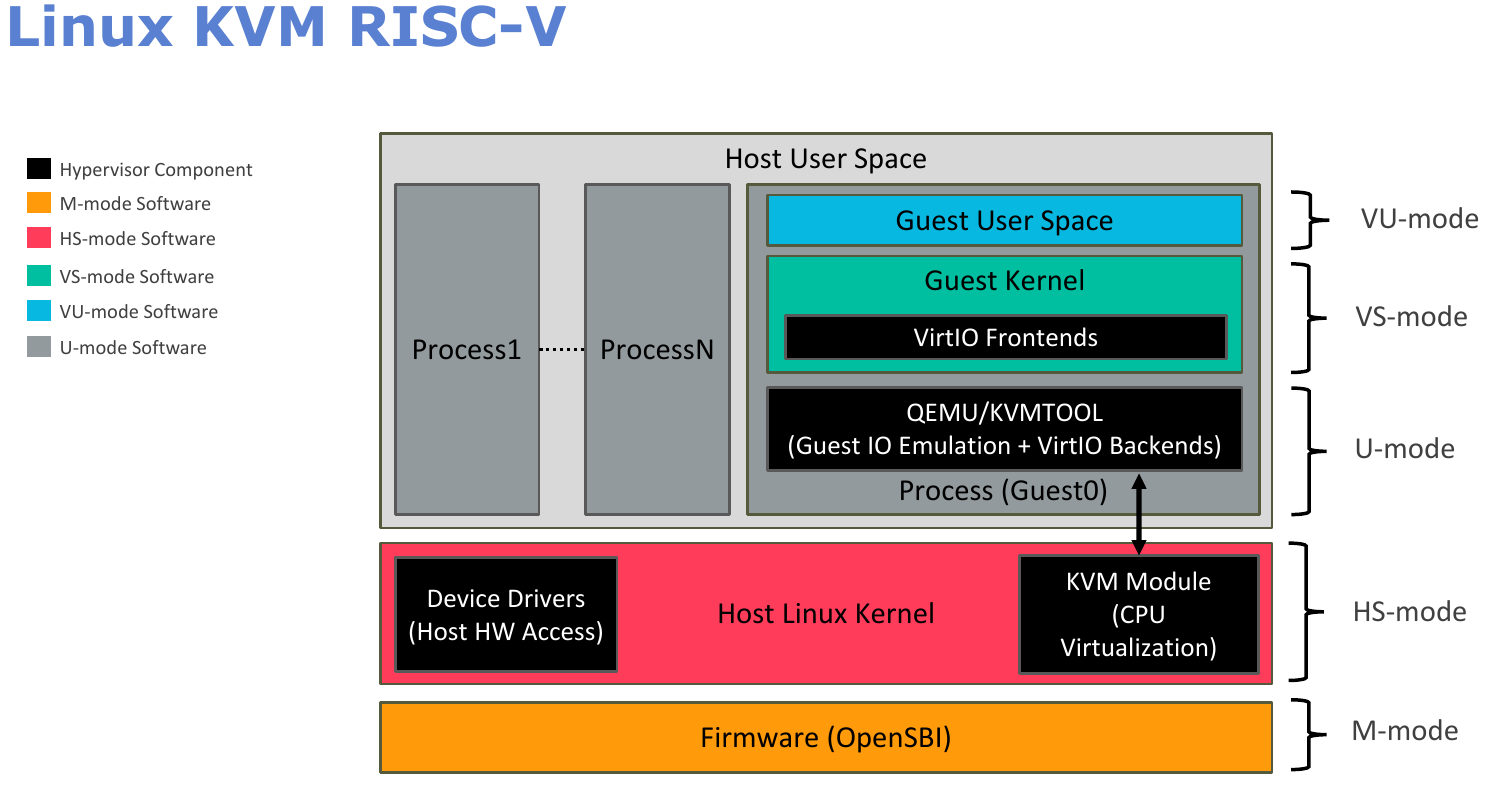
\includegraphics[width=.9\textwidth]{rv-kvm-linux}
	
\end{frame}
%-------------------------------------------------
%-------------------------------------------------


\end{document}